\documentclass[11pt,a4paper]{article}

% Encoding & fonts
\usepackage[utf8]{inputenc}
\usepackage[T1]{fontenc}
\usepackage{mathptmx} % Times New Roman — matches Deliverable 1

% Layout — tight margins for 3-page constraint
\usepackage[top=1.5cm, bottom=1.2cm, left=1.8cm, right=1.8cm]{geometry}
\usepackage{microtype}
\usepackage{parskip}
\setlength{\parskip}{3pt}
\setlength{\parindent}{0pt}

% Graphics & tables
\usepackage{graphicx}
\usepackage{booktabs}
\usepackage{tabularx}
\usepackage{multirow}
\usepackage{enumitem}
\setlist{nosep, leftmargin=1.2em}

% Section formatting — compact (matches Deliverable 1)
\usepackage{titlesec}
\titleformat{\section}{\normalsize\bfseries}{}{0em}{}
\titlespacing*{\section}{0pt}{8pt}{3pt}
\titleformat{\subsection}{\small\bfseries}{}{0em}{}
\titlespacing*{\subsection}{0pt}{5pt}{2pt}

% Euro symbol
\usepackage{eurosym}

% Hyperlinks (invisible)
\usepackage{hyperref}
\hypersetup{hidelinks}

% Colored box for appendix TOC
\usepackage{tcolorbox}
\tcbuselibrary{skins}

% Include external PDFs
\usepackage{pdfpages}

% Header/Footer
\usepackage{fancyhdr}
\pagestyle{fancy}
\fancyhf{}
\fancyfoot[C]{\small\thepage}
\renewcommand{\headrulewidth}{0pt}

\begin{document}

% ── HEADER (matches Deliverable 1) ────────────────────────
\noindent
\begin{minipage}[c]{0.25\textwidth}
    
\includegraphics[width=3.5cm]{artiso-logo.pdf}
\end{minipage}%
\hfill
\begin{minipage}[c]{0.72\textwidth}
    \raggedleft
    \small
    ESADE Entrepreneurial Finance --- CFO of a New Venture\\[1pt]
    {\small Roxane Balsh\"usemann, Christian Nikolov, Mart\'i Lombarte, Leonor Ascen\c{c}\~ao, Tam\'as Fenyvesi}\\[1pt]
    {\small April 9, 2026 --- Final Deliverable}
\end{minipage}

\vspace{4pt}
\noindent\rule{\linewidth}{0.4pt}

% ══════════════════════════════════════════════════════════
% 1. EXECUTIVE RECOMMENDATION
% ══════════════════════════════════════════════════════════
\section{Executive Recommendation}

We recommend raising \textbf{\euro{}3.0\,M pre-seed now} at \textbf{\euro{}27\,M pre-money / \euro{}30\,M post-money} using a blended funding stack: \euro{}1.5--2.0\,M VC + \euro{}0.3--0.5\,M angels/SAFEs + \euro{}0.7--1.2\,M non-dilutive (ENISA/CDTI/ACCI\'O). The valuation is supported by a 5-method triangulation (range: \euro{}21.4--51.4\,M).

The blended structure reduces total dilution from 10\% (pure equity) to 6--8\%, preserving founder ownership at 26.7\% each post-round. Over 40\% of the round comes from non-dilutive sources. This is the fastest path to Series~A from a position of strength, backed by pilot revenue (\euro{}60\,K+ from Deichmann, TATA, NF\&TA), 200+ brand waitlist, 82\% gross margins, and 7 paying logos.

The recommended capital stack is not merely additive; it is structurally sequenced to maximise non-dilutive coverage before the equity tranche prices: ENISA filed in Month~1 as a credibility signal, angel SAFEs deployed in Month~1--2 as bridge, the VC process run in Month~2--4 with ENISA approval in hand, and CDTI/ACCI\'O layered in Month~2--6 in parallel. The non-dilutive tranche (\euro{}0.7--1.2\,M) saves founders 2--5 percentage points of ownership that would otherwise be surrendered to equity investors. At \euro{}27\,M pre-money, investors receive compelling returns (85.7\% IRR, 11.9$\times$ MOIC at 10$\times$ ARR exit) while founders retain majority control through Series~A. By layering non-dilutive instruments underneath the equity raise, we structurally minimise dilution: 6--8\% blended vs.\ 10\% for pure equity. Less dilution today compounds through Series~A and exit, preserving more value for the founding team.

% ══════════════════════════════════════════════════════════
% 2. FINANCIAL NEEDS BY SCENARIO
% ══════════════════════════════════════════════════════════
\section{Financial Needs by Scenario}

Our financial model projects three scenarios across the 5-year horizon. The base case is the operating plan; upside and downside scenarios stress-test the assumptions that drive the most variance in outcomes.

\vspace{-2pt}
\begin{table}[h!]
\centering
\scriptsize
\begin{tabularx}{\textwidth}{p{3.4cm}XXX}
\toprule
\textbf{Metric} & \textbf{Base Case} & \textbf{Upside} & \textbf{Downside} \\
\midrule
Initial funding need & \euro{}3.0\,M & \euro{}3.0\,M & \euro{}3.0\,M \\
FY2030 Revenue & \euro{}36.5\,M & \euro{}148.5\,M & \euro{}3.8\,M \\
FY2030 EBITDA & +\euro{}8.2\,M & +\euro{}55.9\,M & $-$\euro{}2.4\,M \\
Installed base FY2030 & 360 brands & 588 brands & 154 brands \\
Cash floor (lowest point) & $-$\euro{}379\,K (Q4 2028) & $-$\euro{}82\,K (Q4 2026) & $-$\euro{}6.9\,M (Q4 2030) \\
EBITDA breakeven timing & Q4 2028 & Q2 2028 & Never within horizon \\
Series~A timing & Q4 2027 & Pull forward to Q3 2027 & Delay; prepare bridge \\
Series~A size estimate & \euro{}10\,M at 10--15$\times$ ARR & \euro{}15--20\,M at premium & Emergency bridge needed \\
Contingency action required & Execute plan as modeled & Accelerate hiring \& GTM & Activate cost cuts at \euro{}500\,K \\
Management response & Monthly model recalib. & Scale team ahead of plan & Defer 3 hires, cut S\&M 30\% \\
\bottomrule
\end{tabularx}
\end{table}
\vspace{-2pt}

In the \textbf{downside scenario} (conversion rates halved, churn doubled, pricing reduced), the company never reaches EBITDA breakeven and cash deteriorates to $-$\euro{}6.9\,M by Q4~2030 without intervention. The \euro{}500\,K cash trigger activates the contingency plan early: defer 3 planned hires, cut S\&M by 30\%, and reduce monthly burn from \textasciitilde\euro{}120\,K to \textasciitilde\euro{}80\,K, extending runway by \textasciitilde5 months. In the \textbf{upside scenario} (higher pricing, faster enterprise adoption, NRR above 115\%), revenue reaches \euro{}148.5\,M by FY2030 with \euro{}55.9\,M EBITDA, enabling an earlier and larger Series~A at a significant premium. The wide range between scenarios underscores the model's sensitivity to commercial execution. Enterprise NRR and lead growth rate are the two dominant levers. We note that the 200+ brand waitlist has not been validated at conversion, and the cross-sell rates (8\% M2 adoption per period) are benchmarked from PLG SaaS, not from ARTISO's own 7-logo sample; our downside scenario stress-tests both assumptions. Tax loss carry-forward shields \euro{}2.24\,M in cumulative losses through the pre-profitability period.

\vspace{-2pt}
\begin{table}[h!]
\centering
\scriptsize
\begin{tabularx}{\textwidth}{p{2.4cm}XXXXX}
\toprule
\textbf{Metric} & \textbf{FY2026} & \textbf{FY2027} & \textbf{FY2028} & \textbf{FY2029} & \textbf{FY2030} \\
\midrule
Revenue & \euro{}1.2\,M & \euro{}4.3\,M & \euro{}14.1\,M & \euro{}25.7\,M & \euro{}36.5\,M \\
Gross Margin & 82.1\% & 82.1\% & 82.2\% & 82.2\% & 82.3\% \\
EBITDA & (\euro{}755\,K) & (\euro{}973\,K) & (\euro{}357\,K) & +\euro{}3.03\,M & +\euro{}8.22\,M \\
Installed Base & 35 & 81 & 181 & 279 & 360 \\
ARR (EoY) & \euro{}2.1\,M & \euro{}6.4\,M & \euro{}16.1\,M & \euro{}26.2\,M & \euro{}35.7\,M \\
Cash Balance & \euro{}2.08\,M & \euro{}743\,K & (\euro{}379\,K) & \euro{}1.66\,M & \euro{}7.11\,M \\
\bottomrule
\end{tabularx}
\end{table}
\vspace{-4pt}

D\&A is zero at this stage as all infrastructure is cloud-based OpEx with no capitalised development; this would change post-Series~A as the engineering team scales.

% ══════════════════════════════════════════════════════════
% 3. FINANCING ALTERNATIVES
% ══════════════════════════════════════════════════════════
\section{Financing Alternatives}

\subsection{A. Venture Capital (Primary --- \euro{}1.5--2.0\,M)}

Target European B2B SaaS/AI specialists with pre-seed/seed mandates: \textit{Nauta Capital} (Barcelona, B2B SaaS/AI focus, \euro{}1--3\,M tickets), \textit{Inveready} (Barcelona, deep tech), \textit{Samaipata} (Madrid, digital platforms). At \euro{}27\,M pre-money, the lead VC takes 5--7\% for \euro{}1.5--2.0\,M. ARTISO's pilot revenue, 200+ brand waitlist, 82\% gross margins, and cluster GTM model (MODACC, NF\&TA) align with these investors' thesis. Fashion-strategic options include \textit{C4 Ventures} (Milan) and LVMH \textit{La Maison des Startups}, though corporate processes typically add 3--6 months. Run a structured 8-week outreach with parallel term-sheet timelines to create competitive tension; target first term sheet by Month~3.

\subsection{B. Angels \& SAFEs (\euro{}300--500\,K)}

ESADE BAN, Keiretsu Forum Europe, and fashion executives (Mango/Inditex alumni) as domain-specific angels. Tickets of \euro{}25--250\,K via SAFEs with a valuation cap at \euro{}27\,M to bridge while the VC process runs. Total dilution: 1--2\%. Deployment timeline: weeks, not months. Angels provide warm introductions to VC leads, accelerating the fundraise. This tranche serves a dual purpose: immediate cash buffer plus signaling value (named industry angels validate the thesis for institutional investors).

\subsection{C. Non-Dilutive (\euro{}700\,K--1.2\,M)}

\begin{itemize}
\item \textbf{ENISA Emprendedores} --- Participative loans up to \euro{}300\,K. No collateral, performance-linked repayment, 2--4 month approval. \textit{Highest priority}: approval signals credibility and de-risks the round for VCs.
\item \textbf{CDTI NEOTEC} --- Non-repayable R\&D grants \euro{}250--400\,K (70\% co-funding for tech startups $<$3 years). Fits ARTISO's AI ontology and fashion-domain model development. Annual call Q1.
\item \textbf{ICF/ACCI\'O} (Catalonia) --- ICF Pime Innova loans \euro{}100\,K--2.2\,M at Euribor + spread. ACCI\'O Startup Capital direct aid up to \euro{}100\,K (non-repayable). Instruments are combinable and stackable with ENISA/CDTI.
\end{itemize}

\subsection{D. Revenue-Based Financing \& Venture Debt (Not Now)}

Revenue-based financing (Capchase, Re:cap, Uncapped): viable post-\euro{}50\,K MRR (est.\ Q1 2027). Non-dilutive but expensive at 15--25\% APR equivalent; suitable as bridge capital only. Venture debt (Kreos Capital, Bootstrap Europe): available near EBITDA breakeven (H2 2028), typically sized at 20--30\% of the last equity round. Both instruments are premature today but become relevant as the company approaches Series~A milestones.

% ══════════════════════════════════════════════════════════
% 4. FUNDING STRATEGY + VALUATION
% ══════════════════════════════════════════════════════════
\section{Funding Strategy \& Valuation}

\subsection{Recommended Capital Stack}

\vspace{-2pt}
\begin{table}[h!]
\centering
\small
\begin{tabularx}{\textwidth}{Xrrp{5.2cm}}
\toprule
\textbf{Source} & \textbf{Amount} & \textbf{Dilution} & \textbf{Rationale} \\
\midrule
Lead VC & \euro{}1.5--2.0\,M & 5--7\% & Anchor round, board seat, follow-on \\
Angels / SAFEs & \euro{}0.3--0.5\,M & 1--2\% & Bridge speed; domain expertise \\
Non-dilutive & \euro{}0.7--1.2\,M & 0\% & ENISA + CDTI + ACCI\'O \\
\midrule
\textbf{Total} & \textbf{\textasciitilde\euro{}3.0\,M} & \textbf{8--12\%} & 40\%+ non-dilutive; founders keep 2--4pp more \\
\bottomrule
\end{tabularx}
\end{table}
\vspace{-4pt}

\textbf{Dilution advantage:} With pure equity, founders dilute 10\% (\euro{}3\,M / \euro{}30\,M post-money). With the blended stack, only the equity portion (\euro{}1.8--2.3\,M) dilutes, bringing total dilution to 6--8\%. Over 40\% of the round comes from non-dilutive sources at zero equity cost. The non-dilutive tranche (\euro{}0.7--1.2\,M) saves founders 2--5 percentage points of ownership that would otherwise be given up to investors. If non-dilutive instruments are delayed beyond Month~6, we recommend expanding the VC tranche to \euro{}2.0--2.5\,M and accepting 12--15\% dilution rather than leaving the round undersized.

\subsection{Valuation: \euro{}27\,M Pre-Money / \euro{}30\,M Post-Money}

Justified via 5-method triangulation:

\vspace{-2pt}
\begin{table}[h!]
\centering
\small
\begin{tabularx}{\textwidth}{Xr}
\toprule
\textbf{Method} & \textbf{Implied Valuation} \\
\midrule
FY2026 Revenue (\euro{}1.2\,M) $\times$ 40x multiple & \euro{}49.0\,M \\
FY2026 ARR (\euro{}2.1\,M) $\times$ 20x multiple & \euro{}41.3\,M \\
FY2027 Forward Revenue (\euro{}4.3\,M) $\times$ 5x multiple & \euro{}21.4\,M \\
5-Step VC Method (backward from \euro{}357\,M exit) & \euro{}51.4\,M \\
Comparable transactions (European AI/SaaS pre-seed) & \euro{}27.0\,M \\
\midrule
\textbf{Range} & \textbf{\euro{}21.4--51.4\,M} \\
\bottomrule
\end{tabularx}
\end{table}
\vspace{-4pt}

\euro{}27\,M is defensible within the range, sitting between the forward revenue method (\euro{}21.4\,M) and the VC/ARR methods (\euro{}41--51\,M). The VC method yields \euro{}51.4\,M using a 60\% IRR hurdle; we anchor to \euro{}27\,M, a 47\% discount to the VC-implied valuation, to price in pre-seed execution risk and give investors meaningful upside (85.7\% IRR vs.\ the 60\% hurdle). Multiples are calibrated against European AI/SaaS pre-seed comparables with pilot revenue and $>$80\% gross margins (Dealroom 2025 data). \textbf{Acceptable negotiation floor: \euro{}22--25\,M} if needed for closing speed or syndicate quality. Below \euro{}22\,M, dilution exceeds the value of the capital and founders lose strategic control.

\textbf{Investor returns:} Seed investors earn an implied IRR of \textbf{85.7\%}, far exceeding the typical 60\% hurdle rate for European pre-seed funds. Return multiple: \textbf{11.9$\times$} at a 10$\times$ ARR exit multiple, assuming FY2030 ARR of \euro{}35.7\,M and a \euro{}357\,M exit valuation. Even at a more conservative 6$\times$ ARR exit, the return is 7.1$\times$, well above the 3--5$\times$ threshold that defines a successful pre-seed outcome.

\subsection{Cap Table Evolution}

\vspace{-2pt}
\begin{table}[h!]
\centering
\small
\begin{tabularx}{\textwidth}{Xrrr}
\toprule
\textbf{Shareholder} & \textbf{Pre-Seed} & \textbf{Post-Seed} & \textbf{Post-Series~A} \\
\midrule
Founder 1 (CEO) & 33.3\% & 26.7\% & 24.2\% \\
Founder 2 (CTO) & 33.3\% & 26.7\% & 24.2\% \\
Founder 3 (CPO) & 33.3\% & 26.7\% & 24.2\% \\
ESOP & 0\% & 10.0\% & 9.1\% \\
Seed Investors & 0\% & 10.0\% & 9.1\% \\
Series~A & 0\% & 0\% & 9.4\% \\
\bottomrule
\end{tabularx}
\end{table}
\vspace{-2pt}

Founders retain 26.7\% each (80.0\% combined) post-seed, preserving operational and strategic control. ESOP pool: 10\% (4.5\% allocated to early engineering and sales hires, 5.5\% reserved for Series~A grants), sized to cover 8--10 key hires through Series~A without requiring a top-up. Pre-seed investors: 10\% (1,250,000 new shares at \euro{}2.40/share). Series~A dilution is modelled at 9.4\% for a \euro{}10\,M round at 15$\times$ ARR.

% ══════════════════════════════════════════════════════════
% 5. NEXT STEPS
% ══════════════════════════════════════════════════════════
\section{Next Steps \& Execution Timeline}

\subsection{Fundraising Sequencing (Month 1--6)}

\vspace{-2pt}
\noindent
\scriptsize
\begin{tabularx}{\textwidth}{p{1.8cm}XXX}
\toprule
\textbf{Timeline} & \textbf{Equity Track} & \textbf{Non-Dilutive Track} & \textbf{Internal Track} \\
\midrule
Month 1 & Deploy angel SAFEs (\euro{}100--200\,K) & File ENISA application & Data room preparation \\
Month 1--2 & VC outreach begins (Nauta, Inveready, Samaipata) & ENISA under review & Pitch deck finalisation \\
Month 2--4 & VC due diligence \& term sheets & File CDTI NEOTEC + ACCI\'O & Monthly cash monitoring \\
Month 4--5 & Close lead VC (\euro{}1.5--2.0\,M) & ENISA approval expected & Board formation \\
Month 5--6 & Syndicate fill (if needed) & CDTI/ACCI\'O disbursement & Hiring plan activation \\
\bottomrule
\end{tabularx}
\normalsize
\vspace{2pt}

\subsection{Priority Actions}

\begin{enumerate}
\item \textbf{Launch VC process immediately} with a focused target list (Nauta Capital, Inveready, Samaipata). Run a structured 8-week outreach with parallel term-sheet timelines to create competitive tension. Prepare a data room including the financial model, pitch deck, product demo access, and pilot case studies (Deichmann, TATA). Target first term sheet by Month~3.
\item \textbf{Apply for ENISA/CDTI/ACCI\'O in parallel.} Do not wait for grant outcomes before starting the VC process. Non-dilutive capital is additive, not sequential. ENISA approval strengthens the VC pitch by signaling institutional validation. Assign one founder to own the grant pipeline full-time during Months~1--3. CDTI NEOTEC annual call is Q1; file immediately.
\item \textbf{Internal cash trigger at \euro{}500\,K.} If cash balance approaches this threshold, activate contingency: defer 3 planned hires (saving \textasciitilde\euro{}25\,K/mo), cut S\&M by 30\%, and reduce monthly burn from \textasciitilde\euro{}120\,K to \textasciitilde\euro{}80\,K, extending runway by \textasciitilde5 months. The board should review cash position monthly and trigger the plan automatically, without waiting for a vote.
\item \textbf{Begin Series~A preparation Q4 2027.} Target \euro{}10\,M round at 10--15$\times$ ARR. The \euro{}1\,M ARR milestone (est.\ Q3 2027) is the key gate for Series~A readiness. Engage investment bankers or advisors 6 months ahead. Key metrics to present: NRR $>$110\%, LTV/CAC $>$5$\times$, payback $<$12 months, and 30+ installed logos.
\item \textbf{Explore venture debt bridge H2 2028} if Series~A timeline extends beyond plan. Kreos Capital and Bootstrap Europe are relevant lenders at that stage, with facilities typically sized at 20--30\% of the last equity round. Venture debt becomes attractive near EBITDA breakeven when debt serviceability is demonstrable.
\item \textbf{Monthly model recalibration vs.\ actuals.} Revenue, burn, and cash projections must be updated against real data each month. If actuals deviate $>$15\% from the base case, recalibrate scenario thresholds (cash trigger, breakeven timing, hiring pace) and brief the board. Enterprise NRR and lead growth rate are the two variables that most affect outcomes; monitor weekly.
\end{enumerate}

\textbf{Bottom line:} The recommended next step is immediate: launch the VC process and file the ENISA application in parallel this month. The blended funding strategy positions ARTISO to execute its product roadmap, scale the team from 4 to 23, and reach Series~A readiness by Q3 2027 from a position of operational and financial strength.

% ══════════════════════════════════════════════════════════
% APPENDIX TABLE OF CONTENTS
% ══════════════════════════════════════════════════════════
\vfill
\begin{tcolorbox}[
    colback=gray!5,
    colframe=gray!50,
    boxrule=0.4pt,
    arc=2pt,
    left=6pt, right=6pt, top=4pt, bottom=4pt,
    title={\small\bfseries Appendix Contents},
    coltitle=black,
    fonttitle=\small\bfseries,
    colbacktitle=gray!15
]
\small
\begin{tabularx}{\textwidth}{@{}Xr@{}}
Appendix A --- Deliverable 1: Knowing the Venture & p.\,\pageref{app:A} \\
Appendix B --- Deliverable 2: Financial Analysis & p.\,\pageref{app:B} \\
Appendix C --- Financial Model Summary & p.\,\pageref{app:C} \\
Attached: Original Deliverable 1 PDF & p.\,7 \\
Attached: Original Deliverable 2 PDF & p.\,8--10 \\
\end{tabularx}
\end{tcolorbox}

% ══════════════════════════════════════════════════════════
% APPENDIX A
% ══════════════════════════════════════════════════════════
\newpage
\section*{Appendix A --- Deliverable 1: Knowing the Venture (Mar 17)}
\label{app:A}

\subsection*{Company Overview}
\textbf{ARTISO} --- Agentic AI for Creative Workflows. An AI operating system that learns a brand's visual DNA (silhouettes, colours, materials, style rules) and applies it across the entire creative workflow: concept $\rightarrow$ design $\rightarrow$ tech packs $\rightarrow$ campaign assets. 4-layer proprietary fashion intelligence: Brand DNA, User Memory, Project Context, AI Knowledge.

\textbf{Website:} artiso.ai \quad \textbf{Fundraising target:} \euro{}3\,M pre-seed \quad \textbf{Timeline:} Q1 2026 fundraising

\subsection*{Product \& Technology}
ARTISO's platform is built on a 4-layer proprietary fashion intelligence stack: (1)~\textbf{Brand DNA} --- learns and encodes each brand's visual identity (silhouettes, colour palettes, material preferences, style rules); (2)~\textbf{User Memory} --- adapts to individual designer workflows and preferences over time; (3)~\textbf{Project Context} --- maintains coherence across seasonal collections, campaigns, and SKUs; (4)~\textbf{AI Knowledge} --- domain-specific models trained on fashion ontology, not general-purpose image generation. The platform delivers four core workflows: concept generation, design iteration, tech pack automation, and campaign asset creation. Self-trained models (not fine-tuned general models) create a defensible moat. Seatless credit-based pricing eliminates per-user friction and encourages enterprise-wide adoption.

\subsection*{3-Year Goals}
\begin{itemize}
\item \textbf{Revenue:} MRR target \euro{}250--500\,K within $\sim$18 months; \euro{}1\,M+ ARR by Q3 2027
\item \textbf{Customers:} Short-term $\sim$20 design-led brands (pilots + early SaaS); medium-term 100+ brands across Europe and US; long-term 350+ installed base by FY2030
\item \textbf{Team:} Scale from 4 to 23 people --- product, AI systems, enterprise delivery, sales
\item \textbf{Product:} Brand DNA knowledge layer $\rightarrow$ full creative workflow $\rightarrow$ PLM integration $\rightarrow$ campaign asset generation
\item \textbf{Geography:} Europe first (Spain, Germany, Italy, Nordics), then US market entry via fashion hubs
\end{itemize}

\subsection*{Traction}
Paid pilots with Deichmann (\euro{}8.7\,B revenue), TATA Group (\euro{}1.9\,B), NF\&TA, Nude Project, Natura. $>$\euro{}60\,K revenue from pilots. 200+ brands on waitlist. 10+ enterprise NDAs signed. 7 paying logos. Cluster GTM model validated through MODACC (Catalan fashion cluster) and NF\&TA partnerships, enabling efficient multi-brand penetration within industry ecosystems.

\subsection*{Market Opportunity}
AI-in-fashion market: $\sim$\euro{}1\,B (2024), projected \euro{}4--6\,B by 2030 (CAGR $\sim$25\%). ARTISO targets the creative workflow automation segment where no incumbent has established a full-stack, brand-aware solution. Total addressable market: 15,000+ fashion brands globally with $>$\euro{}10\,M revenue and in-house design teams.

\subsection*{Previous Rounds \& Current Shareholders}
No external funding to date. Bootstrapped by founders. Early revenue from pilot projects. \\
\textbf{3 co-founders, equal split (33.3\% each):} Sarah Iglesias Hiller (CEO --- business development, enterprise sales, fashion industry network), Matthias Brenninkmeijer (CTO --- AI/ML architecture, self-trained model development), Lucas Pastur (CPO --- product design, UX, creative workflow expertise). Employee option pool (10\%) planned for seed round to attract senior engineering and sales talent.

% ══════════════════════════════════════════════════════════
% APPENDIX B
% ══════════════════════════════════════════════════════════
\newpage
\section*{Appendix B --- Deliverable 2: Financial Analysis (Mar 26)}
\label{app:B}

\subsection*{Capital Allocation (Q2 2026 -- H1 2028)}

\begin{tabularx}{\textwidth}{l *{3}{>{\raggedleft\arraybackslash}X} >{\raggedleft\arraybackslash}X}
\toprule
\textbf{Category} & \textbf{Q2--Q4 2026} & \textbf{FY2027} & \textbf{H1 2028} & \textbf{Total} \\
\midrule
Product \& Engineering & \euro{}380\,K & \euro{}890\,K & \euro{}640\,K & \euro{}1.91\,M \\
Sales \& Marketing & \euro{}250\,K & \euro{}710\,K & \euro{}480\,K & \euro{}1.44\,M \\
G\&A incl.\ founder salaries & \euro{}190\,K & \euro{}440\,K & \euro{}330\,K & \euro{}960\,K \\
Infrastructure (cloud/GPU) & \euro{}100\,K & \euro{}130\,K & \euro{}100\,K & \euro{}330\,K \\
\midrule
\textbf{Total Outflows} & \textbf{\euro{}920\,K} & \textbf{\euro{}2.17\,M} & \textbf{\euro{}1.55\,M} & \textbf{\euro{}4.64\,M} \\
\bottomrule
\end{tabularx}

\subsection*{Unit Economics (Base Case, Steady State)}

\begin{tabularx}{\textwidth}{l *{3}{>{\raggedleft\arraybackslash}X}}
\toprule
\textbf{Metric} & \textbf{SME} & \textbf{Large} & \textbf{Enterprise} \\
\midrule
ACV & \euro{}17\,K & \euro{}67\,K & \euro{}155\,K \\
Blended CAC & \euro{}8.5\,K & \euro{}18\,K & \euro{}35\,K \\
LTV (5-yr) & \euro{}68\,K & \euro{}301\,K & \euro{}775\,K \\
LTV/CAC & 8.0$\times$ & 16.7$\times$ & 22.1$\times$ \\
Payback (months) & 6 & 3.2 & 2.7 \\
\bottomrule
\end{tabularx}

\vspace{4pt}

\subsection*{Competitive Landscape}

AI-in-fashion market: $\sim$\euro{}1\,B (2024), projected \euro{}4--6\,B by 2030 (CAGR $\sim$25\%). Key competitors: Refabric/Resleeve (\$1--2\,M, single-user design), CALA ($\sim$\$7\,M, design-to-production), Heuritech ($\sim$\euro{}5\,M, trend prediction), Vue.ai (\$47\,M+, retail e-commerce), Adobe Firefly (general creative), Midjourney (text-to-image). ARTISO's moat: proprietary 4-layer fashion intelligence, self-trained models, seatless credit pricing, compounding switching costs. No competitor combines brand-aware AI generation with full workflow coverage (concept through campaign assets).

\subsection*{Financing Sources Considered}

\textbf{Equity:} Nauta Capital, Inveready, Samaipata (lead VC \euro{}1.5--2\,M); ESADE BAN, Keiretsu Forum (angels \euro{}300--500\,K); Mango/Inditex/PVH (strategic). \textbf{Non-dilutive:} ENISA Emprendedores \euro{}300\,K; CDTI NEOTEC \euro{}250--400\,K; ICF/ACCI\'O \euro{}200--300\,K; EIC Accelerator for Series~A phase. \textbf{Debt:} Revenue-based financing post-\euro{}50\,K MRR; venture debt post-Series~A. Blended stack selected to minimise dilution while maximising runway to Series~A milestones.

\subsection*{Key Risks Identified}

\begin{itemize}
\item \textbf{Customer concentration:} 7 paying logos; loss of a single enterprise account would significantly impact near-term revenue. Mitigation: diversify pipeline across segments and geographies.
\item \textbf{Technology moat erosion:} Adobe/OpenAI could enter fashion-specific AI. Mitigation: deepen proprietary Brand DNA layer and accumulate switching costs through compounding brand data.
\item \textbf{Extended enterprise sales cycles:} 6--9 months typical. Mitigation: cluster GTM (MODACC, NF\&TA) reduces cold outreach and accelerates trust-building.
\item \textbf{Cash runway timing:} lowest point $-$\euro{}379\,K at Q4 2028 in base case. Mitigation: \euro{}500\,K cash trigger activates contingency plan (see Section~5).
\item \textbf{Key-person dependency:} first-time founders. Mitigation: ESOP to recruit senior hires; advisory board for governance.
\item \textbf{Model sensitivity:} Enterprise NRR and lead growth rate are dominant levers ($\pm$20\% NRR swings FY2030 ARR by \euro{}27.9\,M). Mitigation: monthly recalibration, scenario-based planning.
\end{itemize}

% ══════════════════════════════════════════════════════════
% APPENDIX C
% ══════════════════════════════════════════════════════════
\newpage
\section*{Appendix C --- Financial Model Summary}
\label{app:C}

\textbf{9 sheets, 4,575 formulas, 0 errors.} Covers: Assumptions (150 parameters, 3 scenarios), Projections (P\&L monthly Y1, quarterly Y2--5), Cash Flow, Balance Sheet (balanced all periods), Headcount (23 roles), Unit Economics (CAC, LTV, churn, payback, burn multiple, magic number, Rule of 40), Cap Table (pre-seed $\rightarrow$ post-seed $\rightarrow$ Series~A), Valuation (5-Step VC Method, triangulation, IRR 85.7\%).

\subsection*{Model Architecture}

\begin{tabularx}{\textwidth}{lX}
\toprule
\textbf{Sheet} & \textbf{Contents} \\
\midrule
Assumptions & 150 parameters across 3 scenarios (Base, Upside, Downside); pricing tiers, conversion rates, churn, NRR, headcount ramp, cost escalators \\
Projections & P\&L monthly for Y1, quarterly for Y2--5; revenue by segment, COGS breakdown, OpEx by department \\
Cash Flow & Operating, investing, and financing activities; monthly granularity Y1, quarterly Y2--5 \\
Balance Sheet & Assets, liabilities, equity; balanced all periods; accounts receivable/payable modelled \\
Headcount & 23 roles across 5 departments; hiring timeline, salary bands, employer cost 1.30$\times$ \\
Unit Economics & CAC, LTV, LTV/CAC, payback period, churn rates, burn multiple, magic number, Rule of 40 \\
Cap Table & Pre-seed $\rightarrow$ post-seed $\rightarrow$ Series~A; share counts, ownership \%, ESOP allocation \\
Valuation & 5-Step VC Method, revenue multiples, ARR multiples, comps, IRR/MOIC analysis \\
Scenarios & Upside/Downside parameter overrides; sensitivity tornado on NRR, lead growth, churn \\
\bottomrule
\end{tabularx}

\subsection*{Key Assumptions \& Limitations}

Bottom-up revenue model: founder FTEs + AEs $\rightarrow$ deal capacity $\rightarrow$ funnel split $\rightarrow$ module penetration $\rightarrow$ 4 revenue streams. 3-tier pricing (SME \euro{}17\,K / Large \euro{}67\,K / Enterprise \euro{}155\,K ACV). Employer cost 1.30$\times$ (Spanish social security). Tax rate 25\% with loss carry-forward (shields \euro{}2.24\,M cumulative losses).

\textbf{Known simplifications:}
\begin{itemize}
\item Deferred revenue not modelled separately (40\% annual billing assumed collected upfront)
\item Sales cycle parameters defined in Assumptions (F89--91) but not wired into pipeline lag in Projections
\item Headcount frozen at 23 from Q4 2028 (would need scaling in practice beyond this point)
\item FX exposure not modelled (all revenues/costs assumed in EUR)
\item Working capital movements simplified (no detailed accounts receivable ageing)
\end{itemize}

\subsection*{Sensitivity Analysis}

The model's three scenarios produce a wide output range: FY2030 revenue spans \euro{}3.8\,M (downside) to \euro{}148.5\,M (upside), with the base case at \euro{}36.5\,M. The dominant variables are \textbf{Enterprise NRR} and \textbf{lead growth rate}. Secondary levers: conversion rates, average deal size, and churn. The downside scenario (conversion halved, churn doubled, pricing reduced) triggers the \euro{}500\,K cash contingency; the upside scenario (higher pricing, NRR $>$115\%, faster enterprise adoption) enables a premium Series~A.

\vspace{6pt}
The blended funding strategy---anchored by \euro{}0.7--1.2\,M in non-dilutive capital and disciplined VC pricing at \euro{}27\,M pre-money---positions ARTISO to execute its product roadmap, scale the team from 4 to 23, and reach Series~A readiness by Q3 2027. The recommended next step is immediate: launch the VC process and ENISA application in parallel this month.

% ══════════════════════════════════════════════════════════
% ATTACHED: ORIGINAL DELIVERABLE PDFs
% ══════════════════════════════════════════════════════════
\newpage
\vspace{4pt}
\noindent\fbox{\parbox{\textwidth}{\small\textbf{Note:} The following pages reproduce Deliverables 1 and 2 as originally submitted in March 2026. Figures in these historical documents reflect earlier model versions and have since been superseded by the final figures in the main body of this report.}}
\vspace{4pt}

\section*{Attached: Original Deliverable 1 (Mar 17, 2026)}
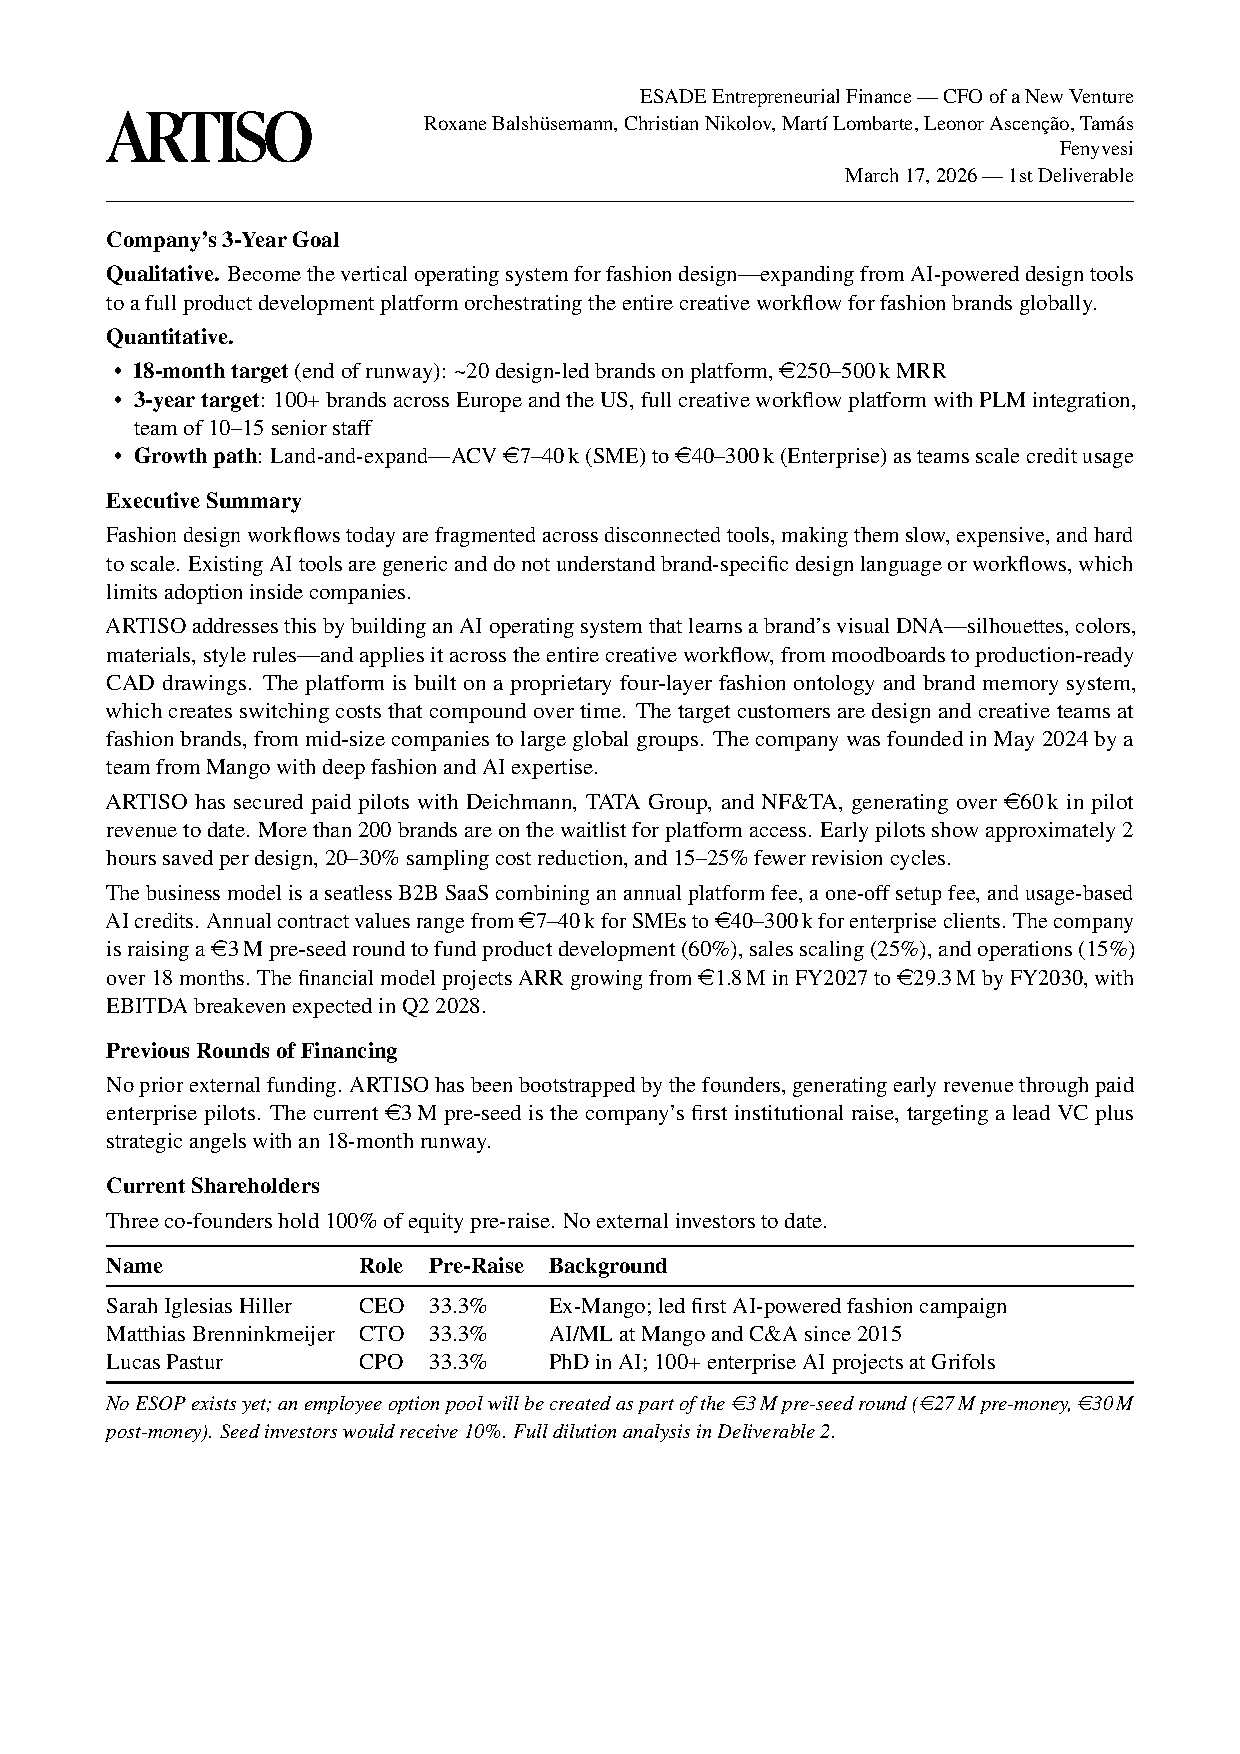
\includepdf[pages=-]{artiso-deliverable-1.pdf}

\section*{Attached: Original Deliverable 2 (Mar 26, 2026)}
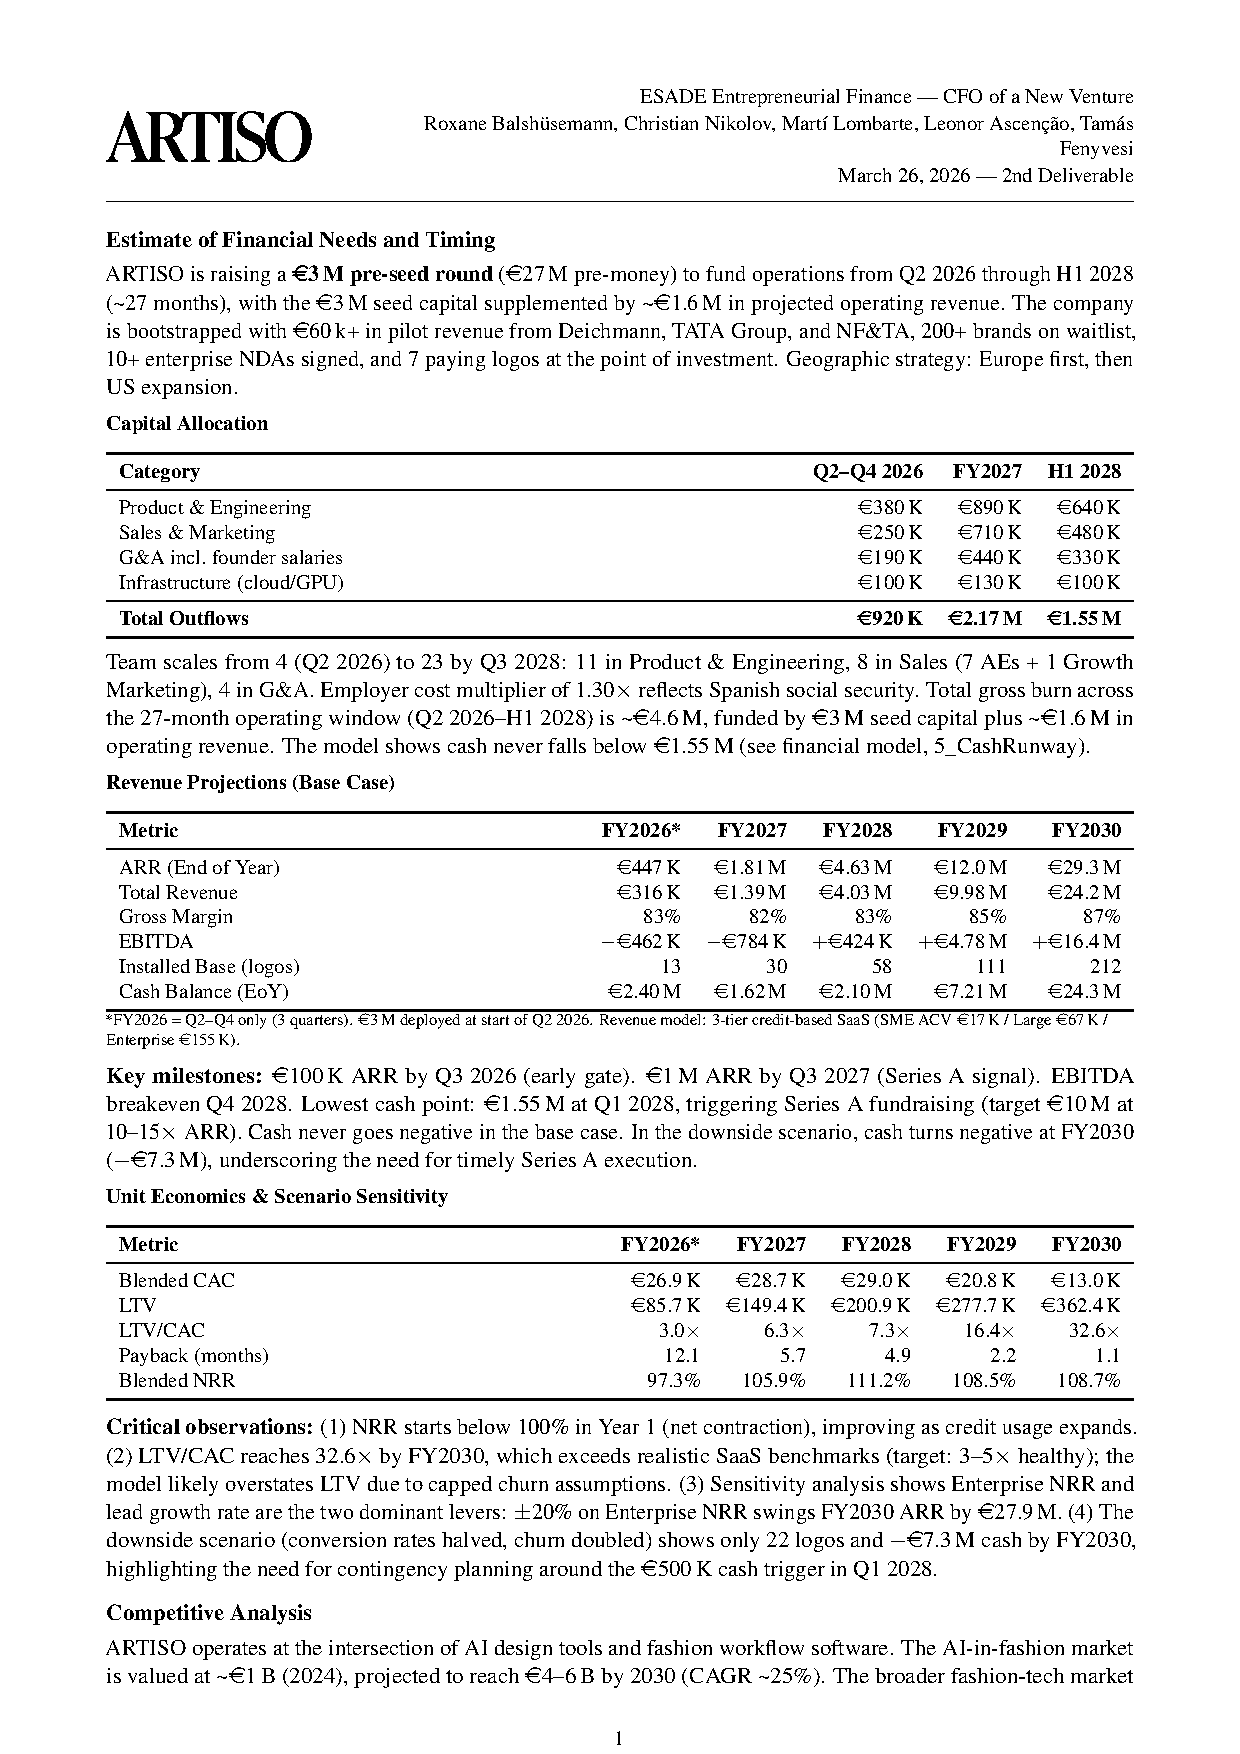
\includepdf[pages=-]{artiso-deliverable-2.pdf}

\end{document}
